% !TEX root = ../article.tex

\section{Results and discussion}

\subsection{Numerical solutions}

On figure \ref{fig:flux0} we can see that the flux has the expected behaviour of a cosine shape, showing a peak at the centre and 0 at the border.
The shape of the flux is not the typical "chopped cosine" since no extrapolated distance was given to the case.
The relative error is very low (below 0.01\%), and as we can see, the numerical solution is indistinguishable from the analytical one.
The effective multiplication factor was also found with very high accuracy, showing an overprediction of 0.3 pcm for the reference mesh.

\begin{figure*}[htbp]
    \centering
    \begin{subfigure}[b]{0.42\textwidth}
        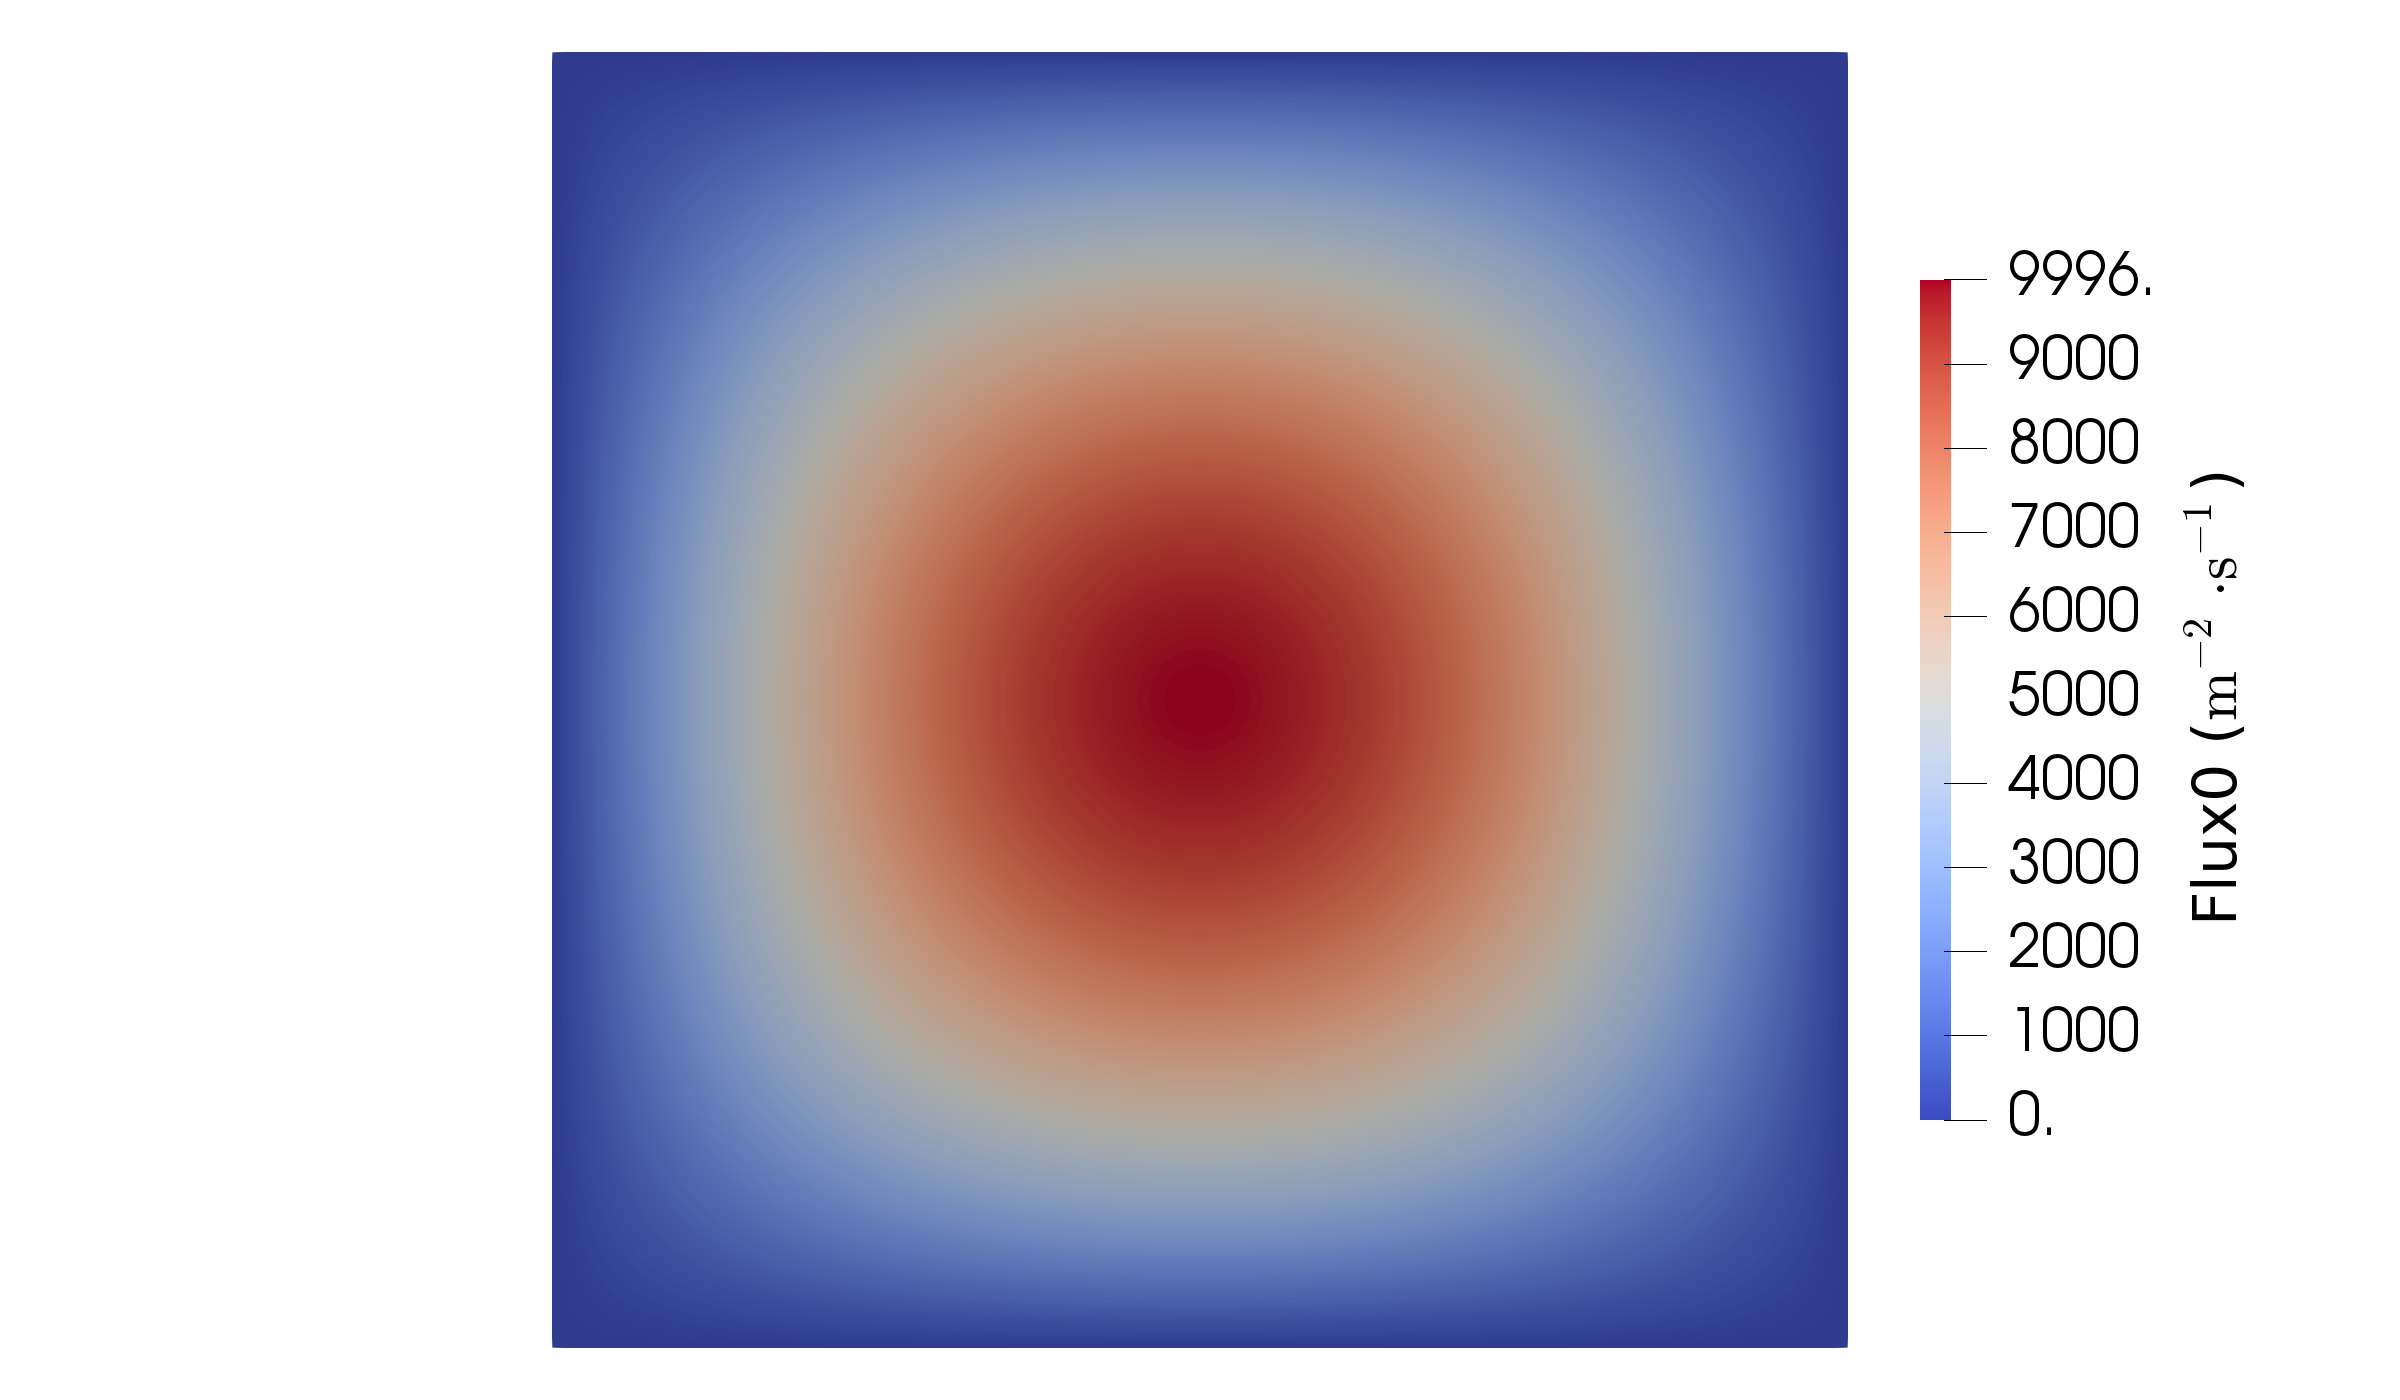
\includegraphics[width=68mm, trim={18cm 0 0 0}, clip]{3_results_and_discussion/figures/flux0.png}
        % \caption{Flux on the domain}
        % \label{fig:flux0Field}
    \end{subfigure}
    \begin{subfigure}[b]{0.56\textwidth}
        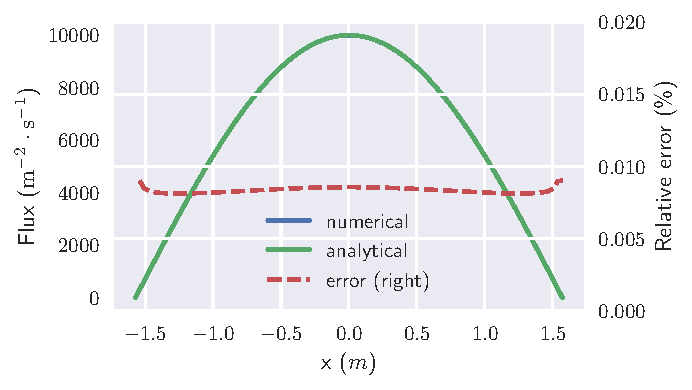
\includegraphics[width=88mm]{3_results_and_discussion/figures/flux0.pdf}
        % \caption{Flux over AA'}
        % \label{fig:flux0AA}
    \end{subfigure}
    \caption{Flux on the domain and results over line AA'}
    \label{fig:flux0}
\end{figure*}

The correct solution of the momentum equation under the conditions of this problem is quite demanding on the divergence discretization scheme of velocity.
A first order upwind scheme fails to generate a correct flow and pressure fields, requiring the use of a second-order upwind scheme with results presented in figures \ref{fig:UMagnitude} and \ref{fig:p}.
It is relevant to mention that the velocity plot in figure \ref{fig:UMagnitude} has a blunt tip in the centre due to the mesh having an even number of cells, therefore there is no cell in the centre of the domain.
A simple test was made with a cell in the centre, offering no benefit to the solution.
With the lack of any benefit, it was decided not to have a cell in the centre to avoid the problem of defining a relative error in the centre of the domain, where the analytical solution to velocity is 0.

The relative error graphic for velocity shows that it peaks quickly and reduces to an approximately constant value away from the boundary.
While a finer mesh at the boundary could appear to offer modest improvements, even though errors are already very low, this improvement was not observed.
A mesh refinement at the walls or a mesh with refinement at the walls and in the centre did not convey any improvement over a uniform one.

\begin{figure*}[htbp]
    \centering
    \begin{subfigure}[b]{0.42\textwidth}
        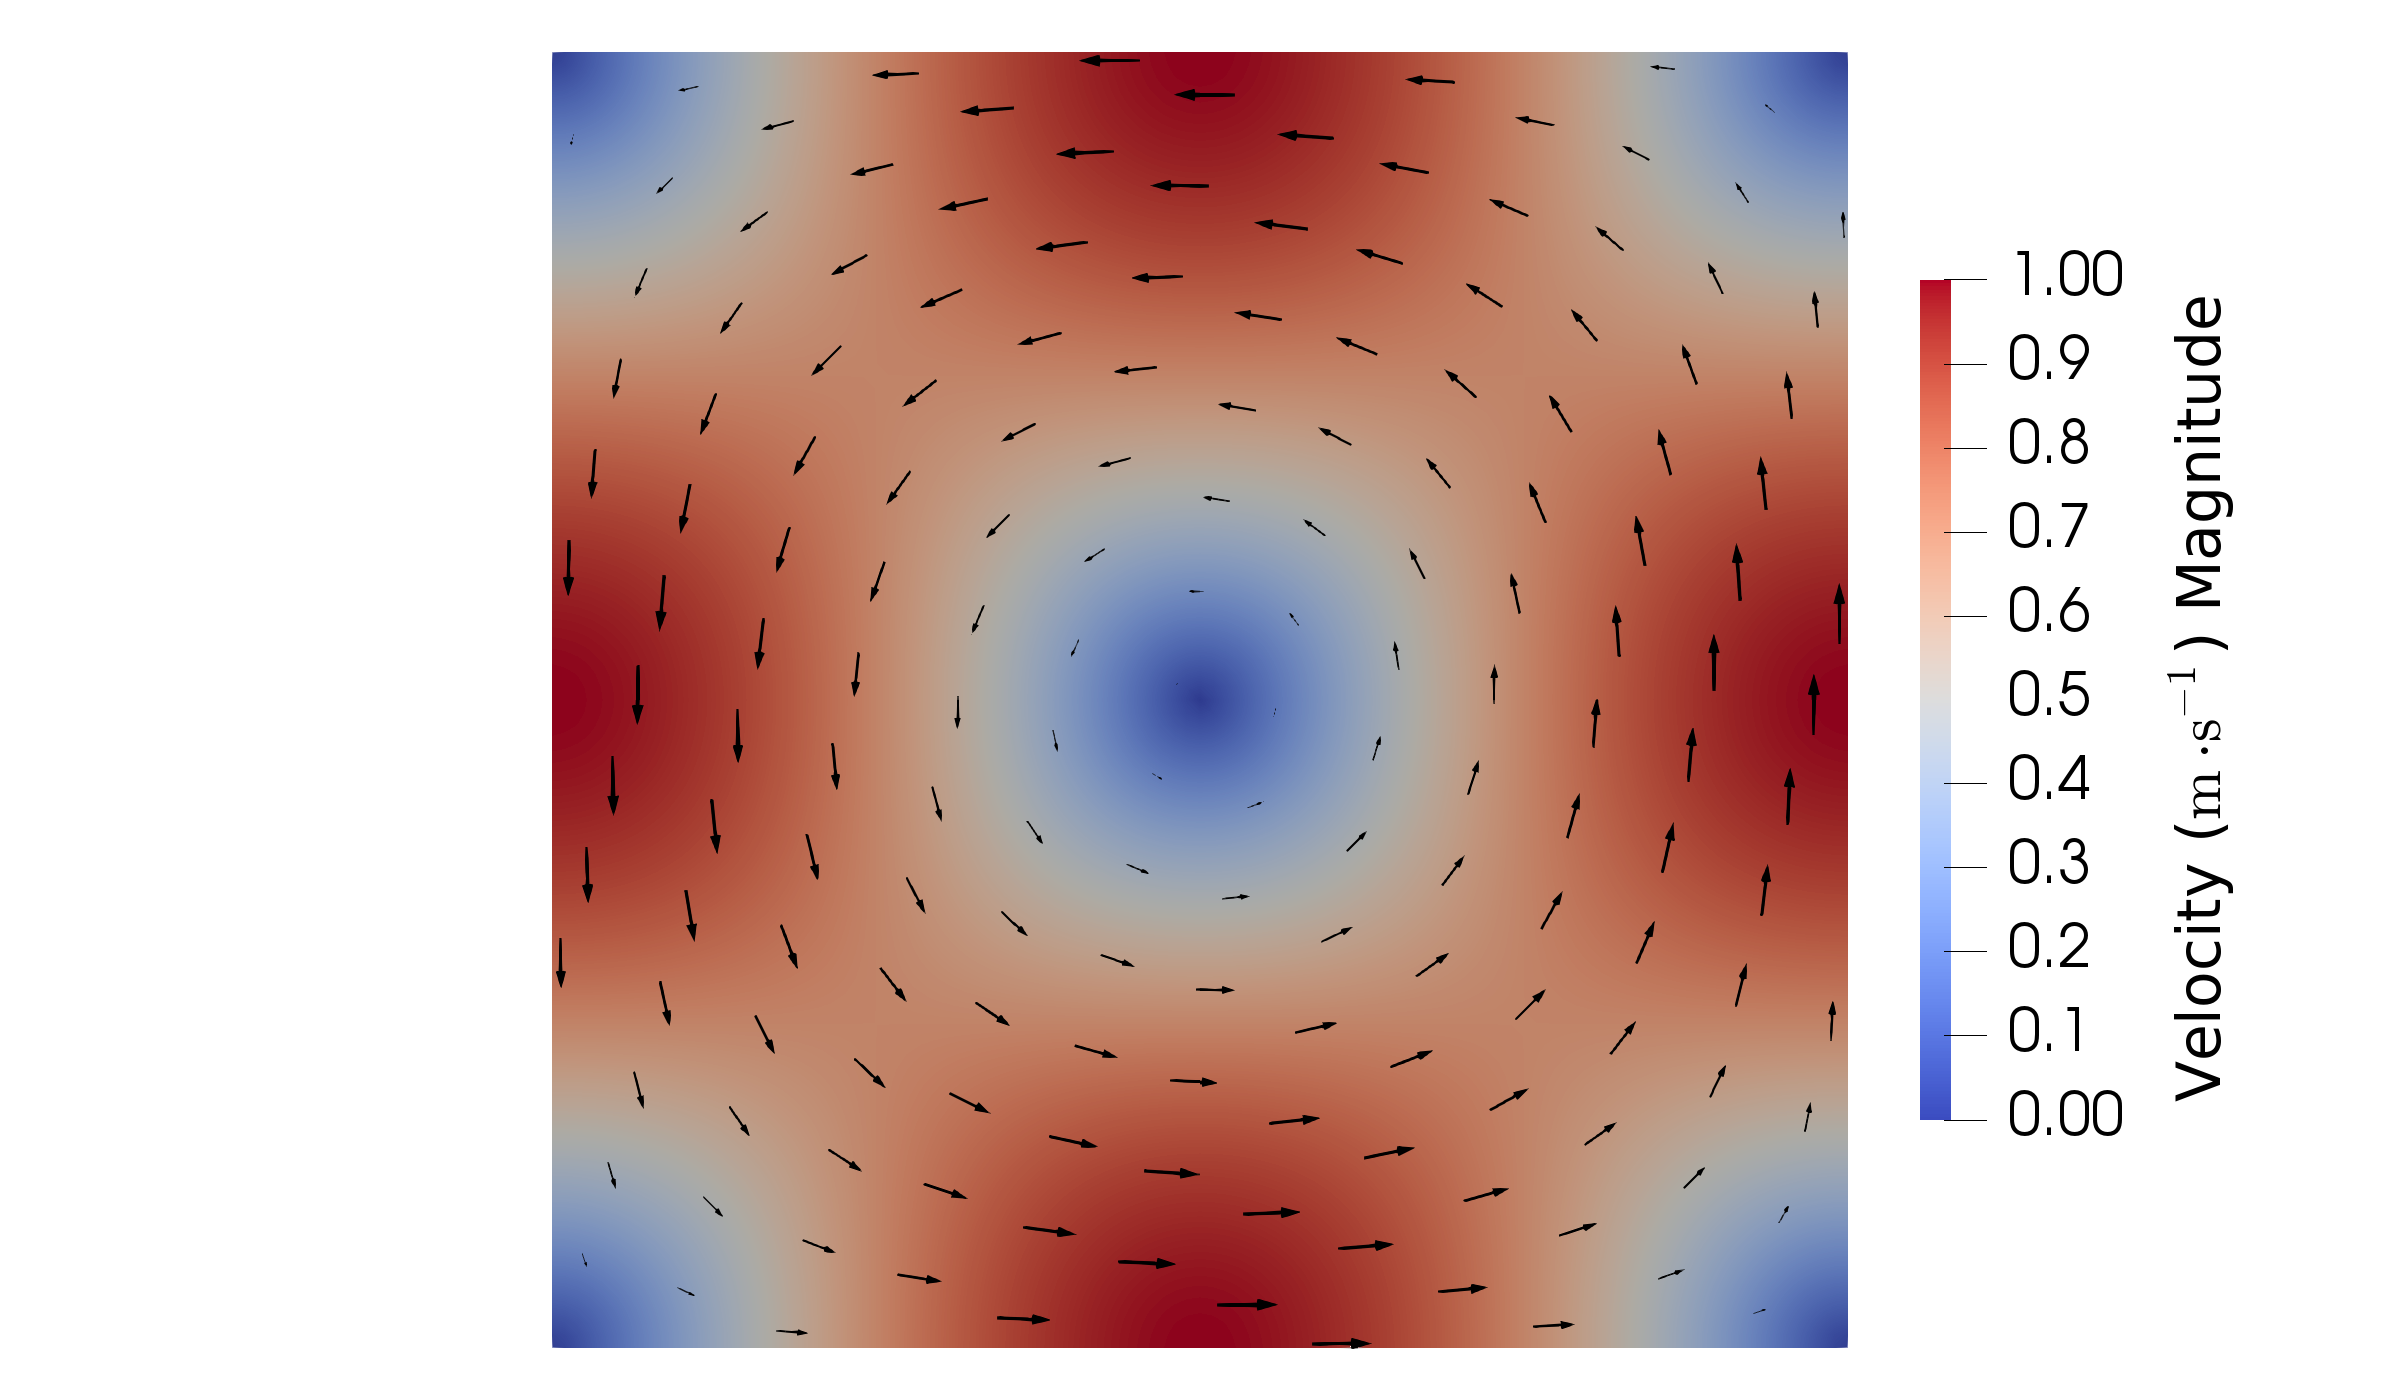
\includegraphics[width=68mm, trim={18cm 0 0 0}, clip]{3_results_and_discussion/figures/UMagnitude_glyph.png}
        % \caption{Velocity magnitude on the domain}
        % \label{fig:UMagnitudeField}
    \end{subfigure}
    \begin{subfigure}[b]{0.56\textwidth}
        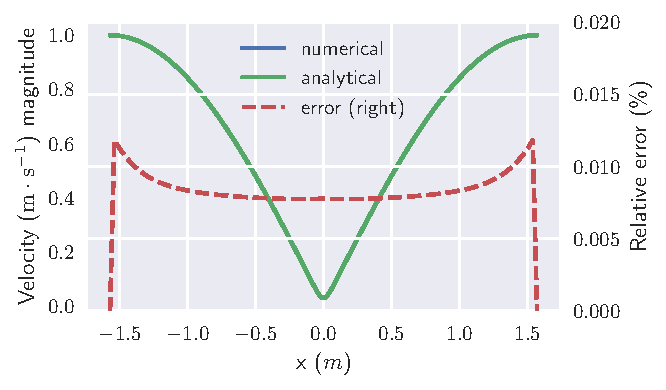
\includegraphics[width=88mm]{3_results_and_discussion/figures/velocity_mag.pdf}
        % \caption{Velocity magnitude over AA'}
        % \label{fig:velmagAA}
    \end{subfigure}
    \caption{Velocity magnitude on the domain and results over line AA'}
    \label{fig:UMagnitude}
\end{figure*}

Pressure has the lowest error, at approximately 0.0001\%, with an unusual curve shape.
Upon closer investigation of the numerical and analytical values, it is clear that the numerical value is higher than the analytical closer to the boundary while the reverse is true for the centre.
Therefore, the zone of 0 error simply represents an intersection where both happen to be equal.

\begin{figure*}[htbp]
    \centering
    \begin{subfigure}[b]{0.42\textwidth}
        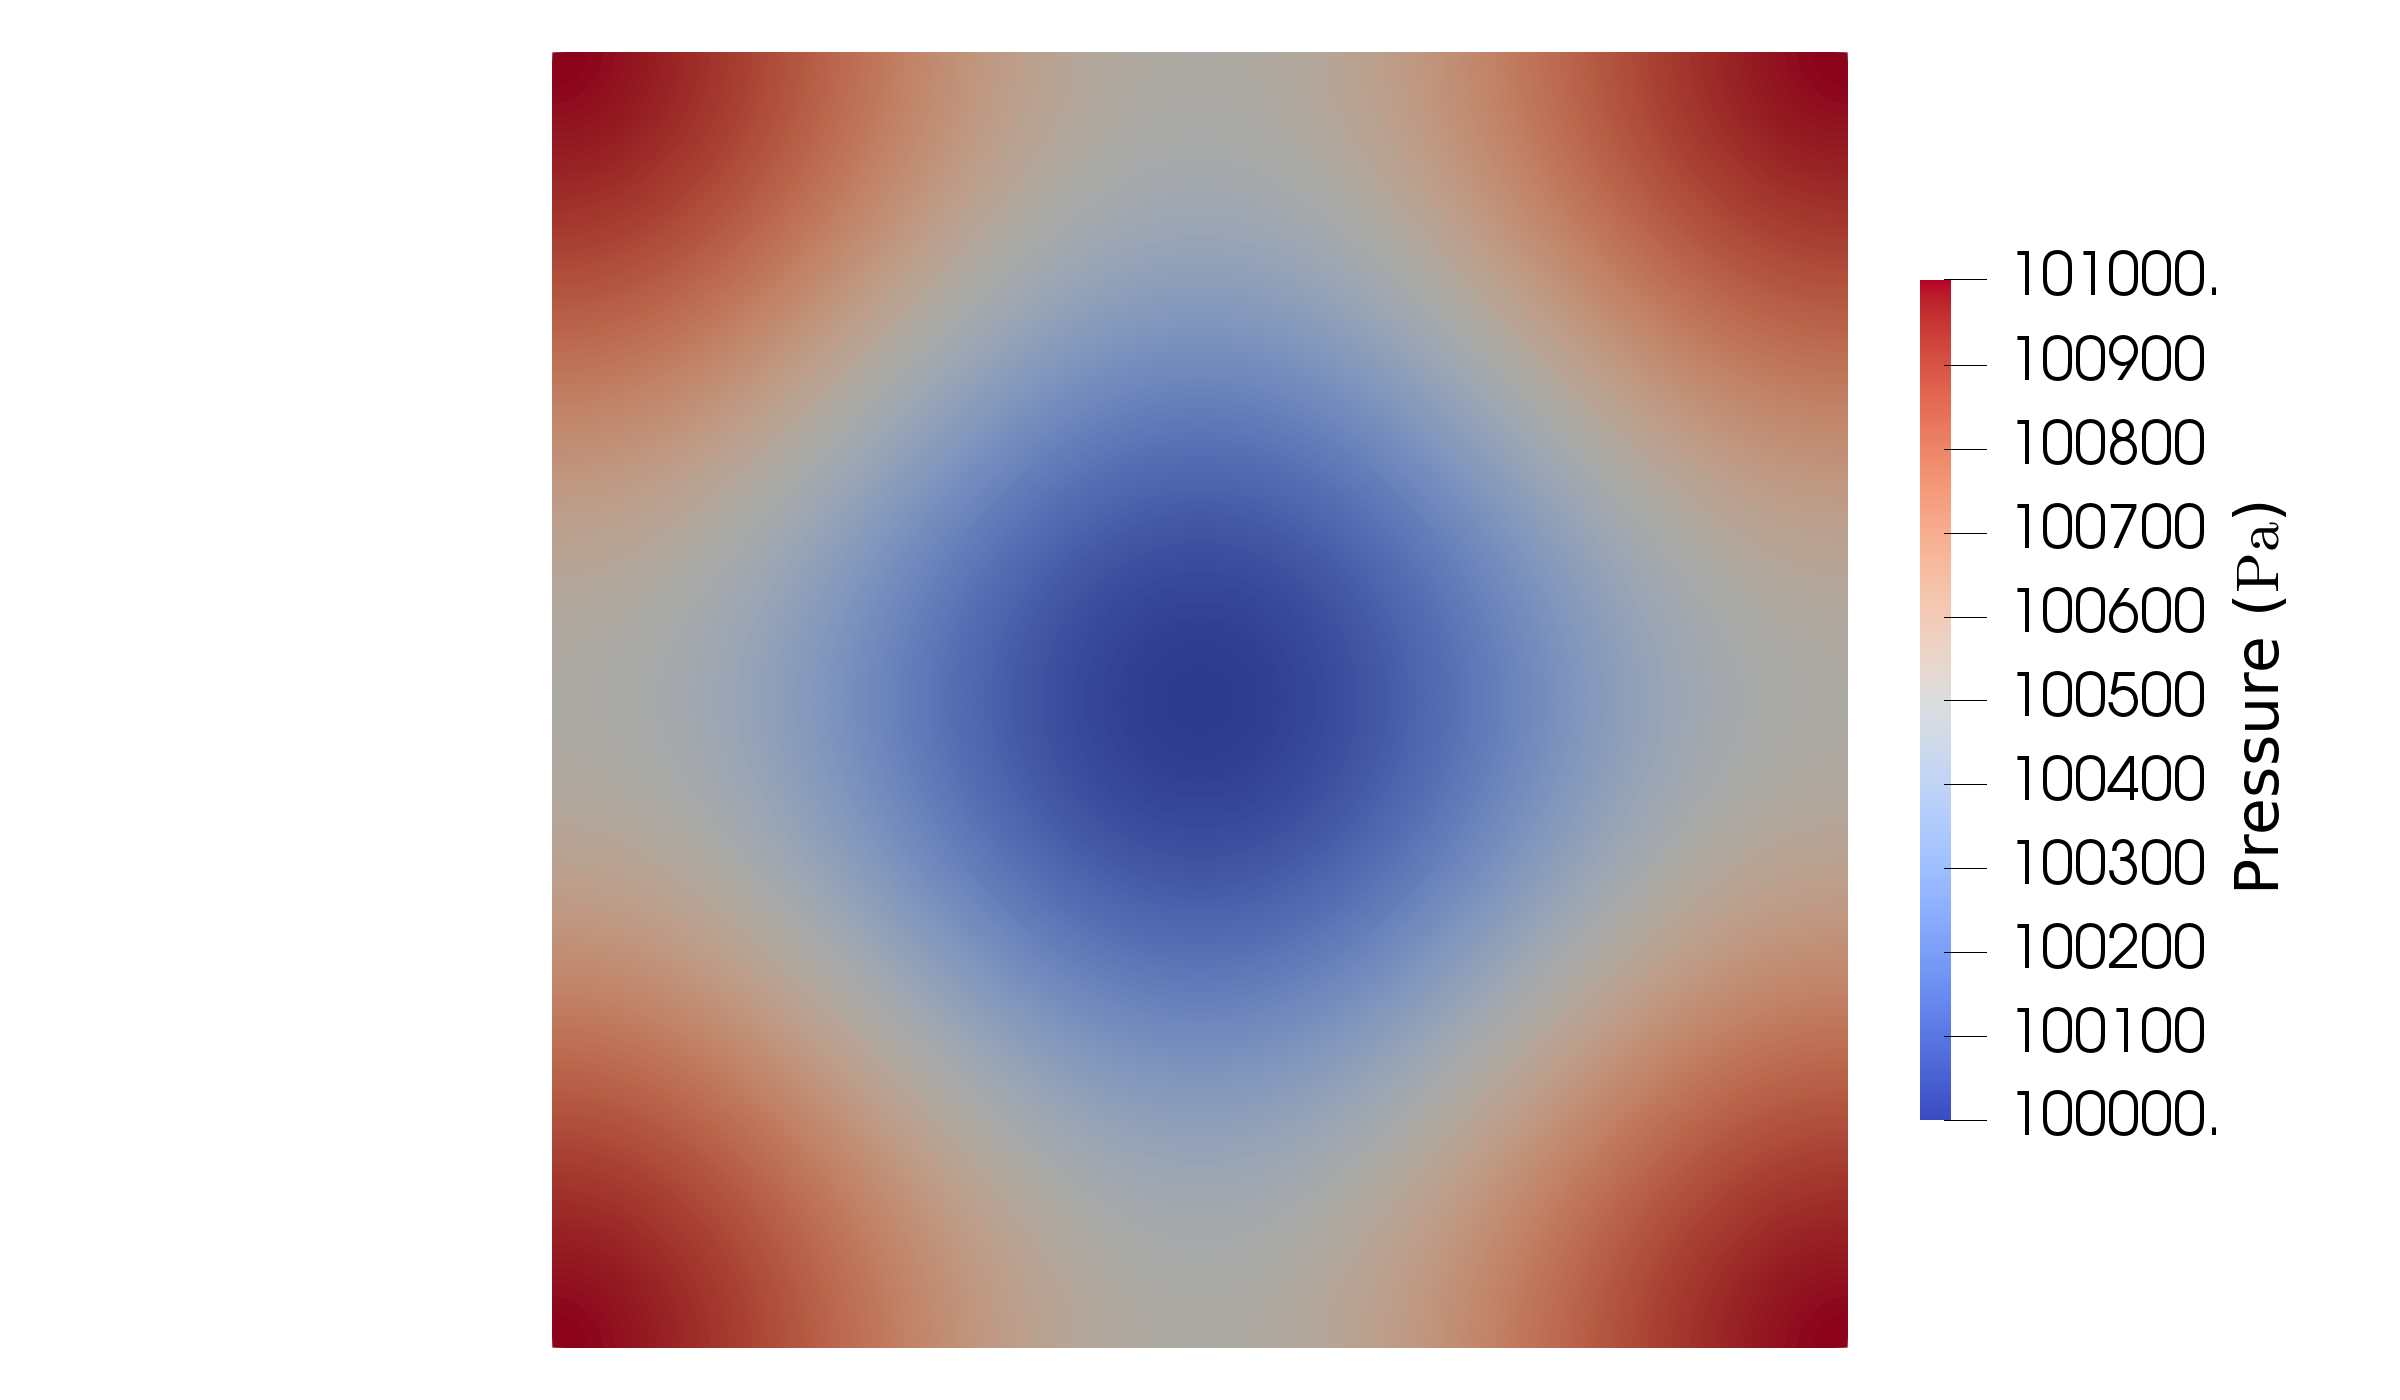
\includegraphics[width=68mm, trim={18cm 0 0 0}, clip]{3_results_and_discussion/figures/p.png}
        % \caption{Pressure on the domain}
        % \label{fig:pField}
    \end{subfigure}
    \begin{subfigure}[b]{0.56\textwidth}
        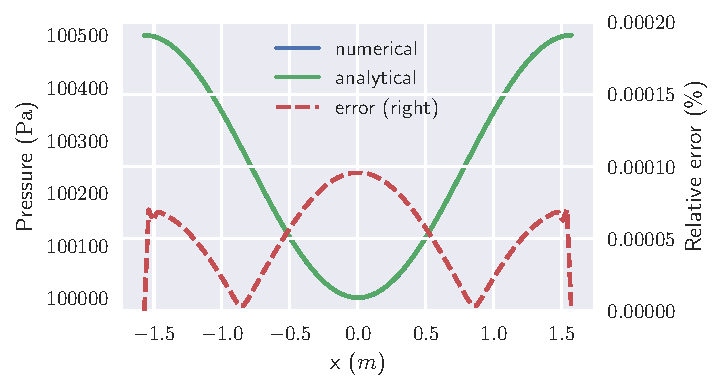
\includegraphics[width=88mm]{3_results_and_discussion/figures/pressure.pdf}
        % \caption{Pressure over AA'}
        % \label{fig:pressureAA}
    \end{subfigure}
    \caption{Pressure on the domain and results over line AA'}
    \label{fig:p}
\end{figure*}

Solving the temperature field reveals some challenging characteristics of this case.
Term dominance can easily be a problem since $ \rho c_{\text{p}} >> k $ usually, resulting in advection strongly dominating over diffusion.
Advection of energy should be analytically 0 for this problem but numerically becomes a very low non-zero number. Multiplying this numerical noise by a relatively big number results in unnaceptable noise levels that prevent the calculation of the correct temperature field.
Despite the temperature field being resolved to a very low relative error as shown at figure \ref{fig:T}, indicating convergence, the error field of this case has a unique shape that is strongly influenced by the advection noise.
Investigating the best way to deal with this problem should be a priority in the future in order to increase the robustness of the proposed case.

\begin{figure*}[htbp]
    \centering
    \begin{subfigure}[b]{0.42\textwidth}
        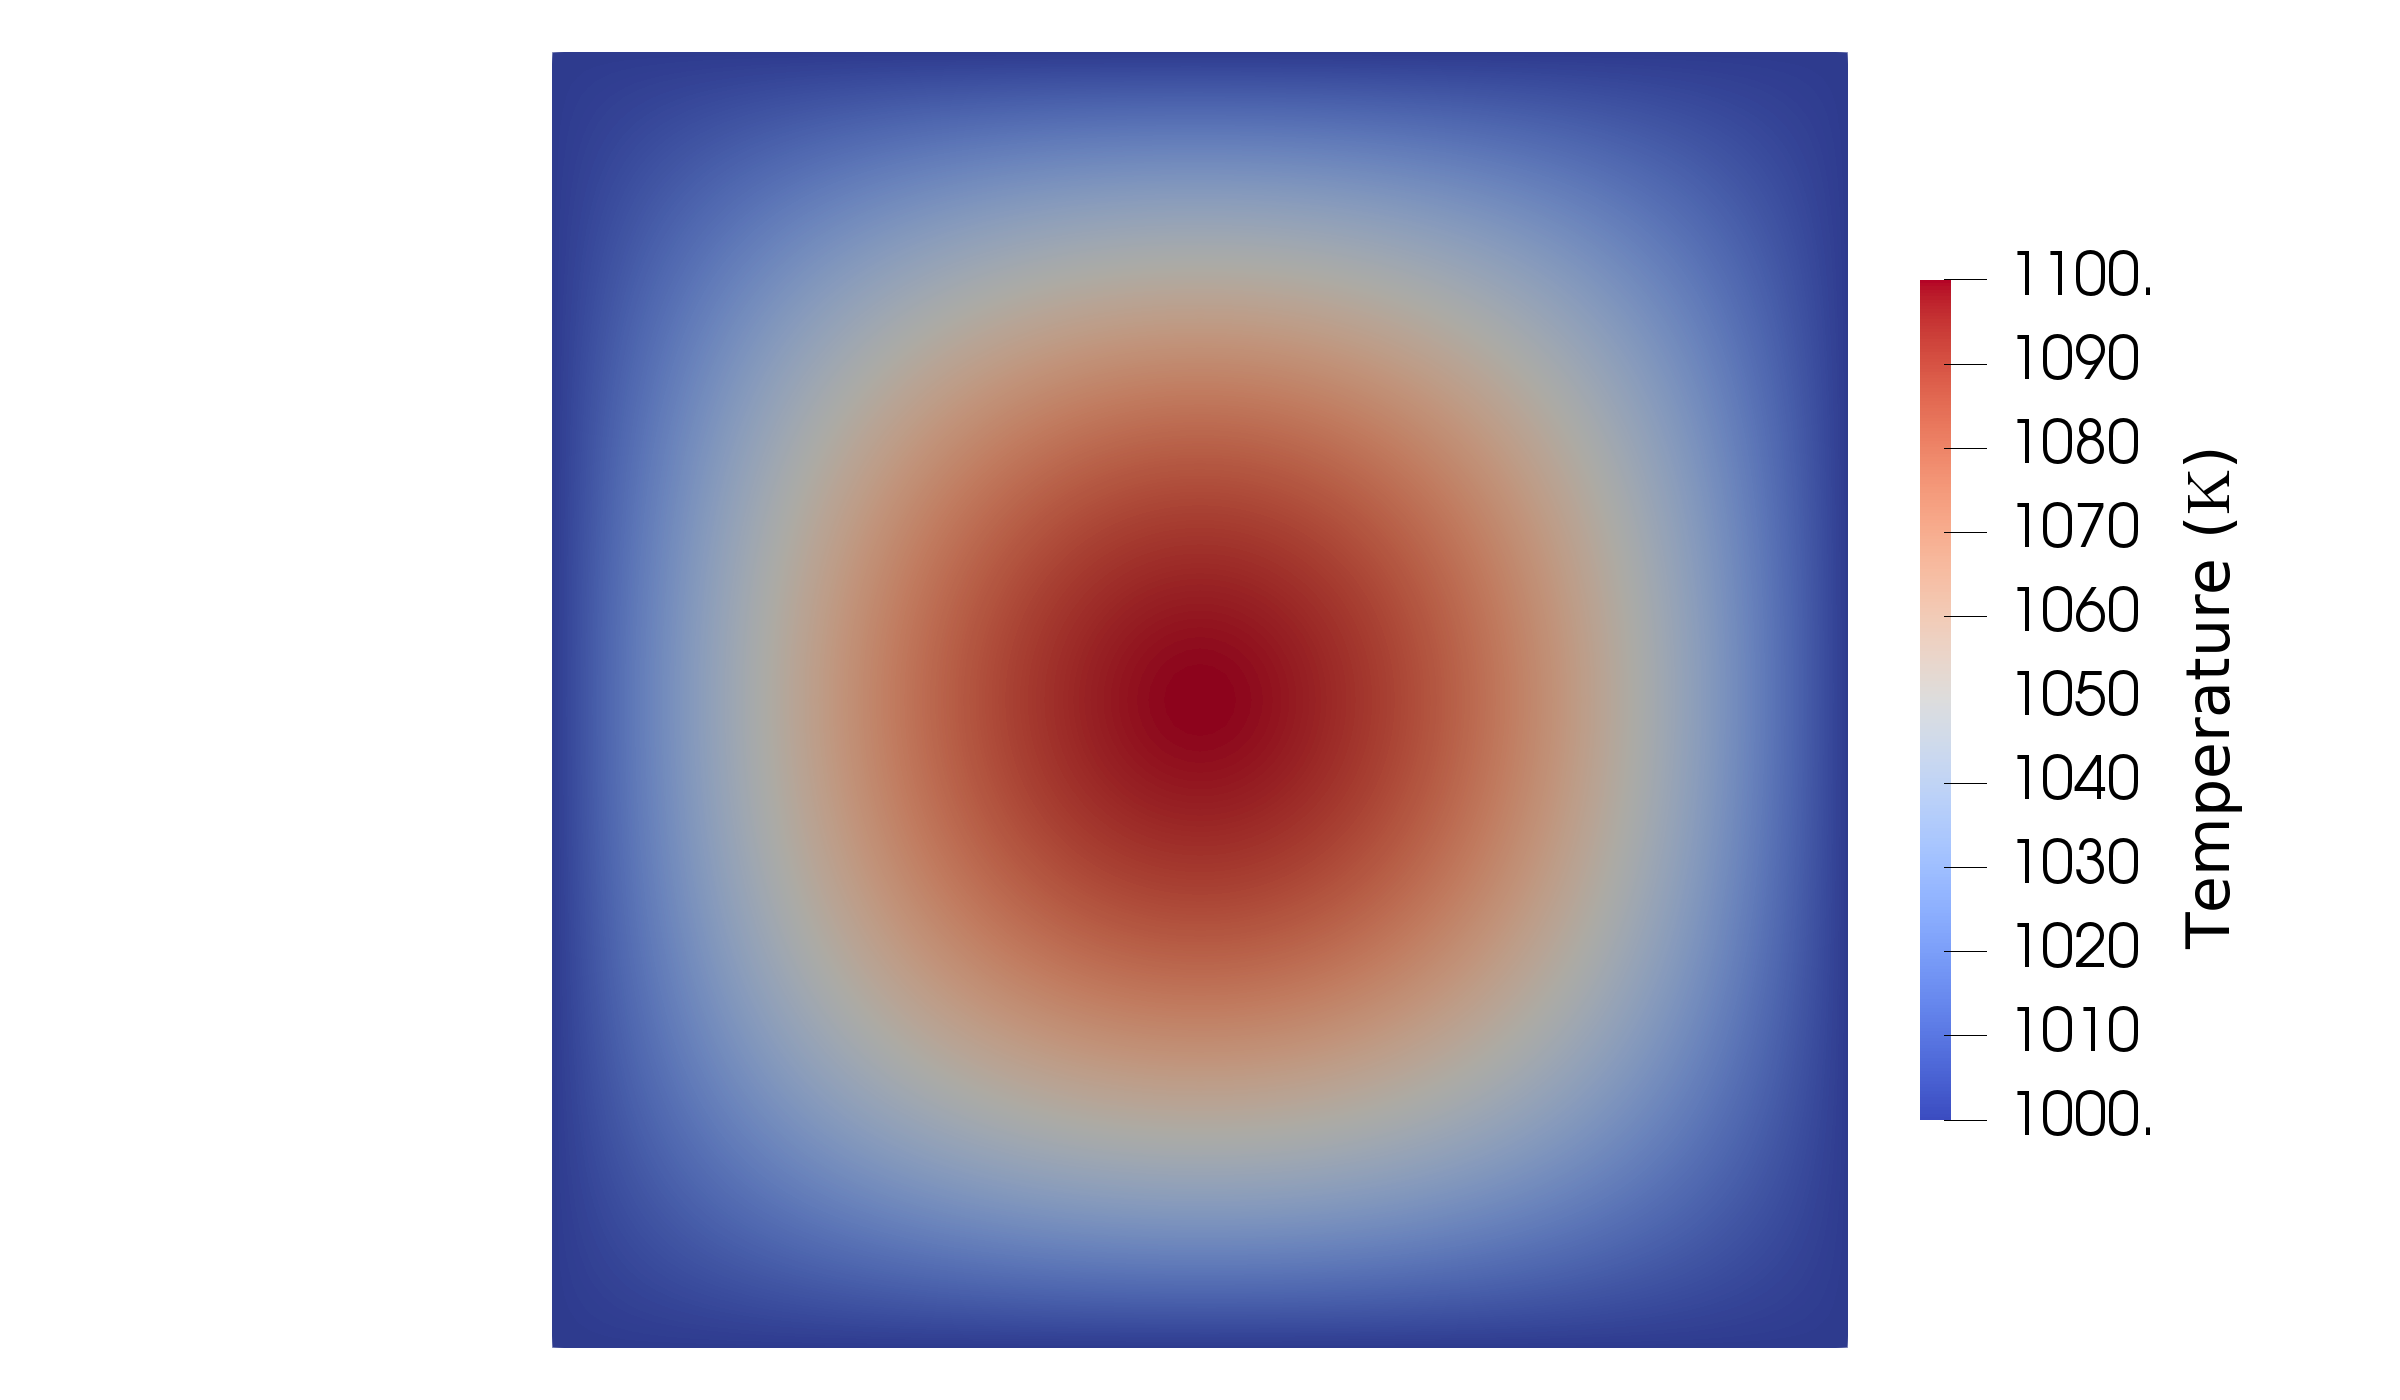
\includegraphics[width=68mm, trim={18cm 0 0 0}, clip]{3_results_and_discussion/figures/T.png}
        % \caption{Temperature on the domain}
        % \label{fig:TField}
    \end{subfigure}
    \begin{subfigure}[b]{0.56\textwidth}
        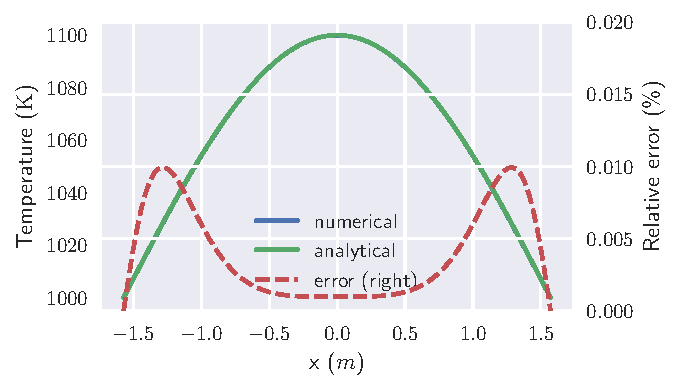
\includegraphics[width=88mm]{3_results_and_discussion/figures/temperature.pdf}
        % \caption{Temperature over AA'}
        % \label{fig:temperatureAA}
    \end{subfigure}
    \caption{Temperature on the domain and results over line AA'}
    \label{fig:T}
\end{figure*}

\subsection{Mesh studies}

Figure \ref{fig:normsU} shows the $ L_{1} $ and $ L_{2} $ norms of velocity on the domain where mesh size indicates the number of uniform cells in the x and y direction.
As can be seen on the figure, the norms decrease quickly with mesh refinement, reaching an assymptotic value at 100 x 100 cells.

\begin{figure}[htbp]
    \centering
    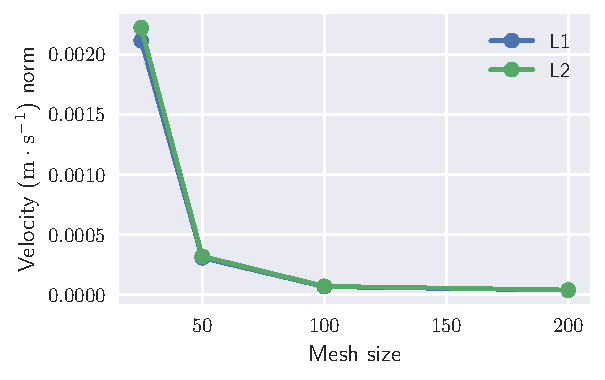
\includegraphics[width=78mm]{3_results_and_discussion/figures/normsU.pdf}
    \caption{$ L_{1} $ and $ L_{2} $ norms for velocity}
    \label{fig:normsU}
\end{figure}

Norms for other variables show a similar trend, also reaching an assymptotic value at 100 cells for each dimension.
Therefore, we consider the mesh converged for this problem.
All graphics presented were created from results of calculation using this mesh.

The increase in wall time from a mesh refinement is significant as shown in figure \ref{fig:wallTime}.
At mesh size 25, the minimum wall time is limited by startup operations, where a mapping of values between the fluid mechanics and neutronics meshes is established, and coded sources and coded boundary conditions are compiled.
At mesh size 200 the wall time is limited by processing power.
At mesh size 50, the case runs at approximately 50 seconds in a common desktop, making it a good candidate for use as a fast regression testing during code development.
At mesh size 100, where mesh is converged, the problem takes only 180 seconds, making it the appropriate resolution for further developments in this problem.

\begin{figure}[htbp]
    \centering
    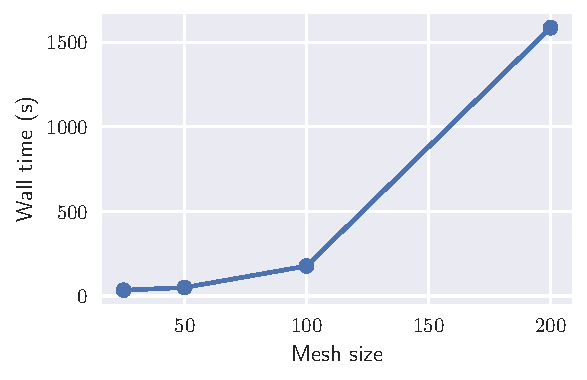
\includegraphics[width=78mm]{3_results_and_discussion/figures/wallTime.pdf}
    \caption{Wall time for different mesh sizes}
    \label{fig:wallTime}
\end{figure}
